\documentclass{article}
\usepackage{polski}
\usepackage[utf8]{inputenc}
\usepackage{graphicx}
\usepackage{float}

\title{Problem pudełek}
\author{Ahmed Abdelkarim, Aleksandra Hernik}
\begin{document}
\maketitle

\section{Instrukcja obsługi}
\begin{figure}[H]
\centering
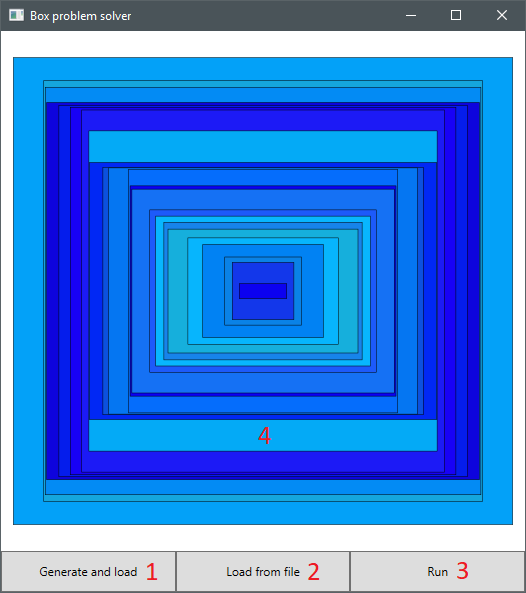
\includegraphics[width=0.8\textwidth]{instrukcja.png}
\caption{Interfejs użytkownika}
\end{figure}
Aby skorzystać z aplikacji, należy najpierw kliknąć na przycisk \textit{Load data} (1) i wybrać plik z danymi wejściowymi. Po zaakceptowaniu pliku pojawi się komunikat o liczbie wczytanych pudełek. Następnie trzeba kliknąć przycisk \textit{Run} (2). W wyniku pojawi się komunikat o długości najdłuższego możliwego ciągu pudełek oraz nazwa pliku wynikowego. Ponadto, w obszarze powyżej guzików (3) zostanie przedstawiona graficzna reprezentacja rozwiązania. Uwaga: wszystkie pudełka są obrócone tak, że dłuższa krawędź to szerokość.  Pudełka są przeskalowane tak, że największe z nich zajmuje całą szerokość okienka.

\section{Opis testów}
\subsection{8 identycznych pudełek}
Dane wejściowe: 8 pudełek, każde o wymiarach 5x10 lub 10x5.

Wynik: lista zawierająca jedno pudełko.

\subsection{9 kwadratowych pudełek}
Dane wejściowe: 9 różnych kwadratowych pudełek, o wymiarach od 1x1 do 9x9 (podanych w losowej kolejności). 

Wynik: Lista zawierająca wszystkie pudełka.
\begin{figure}[H]
\caption{Graficzna reprezentacja wyniku}
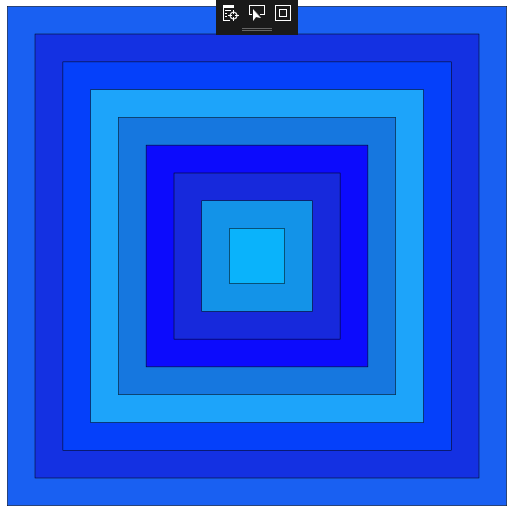
\includegraphics{square_boxes_res.png}
\end{figure}

\subsection{Dwie ścieżki}
Dane wejściowe: 5 pudełek o wymiarach: 11x10, 10x5, 8x6, 7x5, 3x2. W danych istnieją 2 pudełka (8x6 i 10x5), które mieszczą się w większym pudełku, ale nie w sobie nawzajem. Patrząc na pozostałe pudełka można zauważyć, że korzystniejszy jest wybór pudełka o mniejszej powierzchni - 8x6.

Wynik: Aplikacja poprawnie dokonuje wyboru uzyskując w ten sposób ciąg 4-elementowy, zamiast 3-elementowy, jak w przypadku, gdyby zostało wybrane złe pudełko.

\section{Wnioski}

\section{Zmiany w stosunku do dokumentacji wstępnej}
\begin{itemize}
\item Na początku wynikowego pliku dodana jest informacja o długości otrzymanej ścieżki.
\item Dla pliku wejściowego o nazwie \textit{file.ext}, plik wyjściowy nazywa się \textit{file\textunderscore output.txt}.
\end{itemize}

\section{Podział pracy}
Ahmed Abdelkarim zaimplementował interfejs użytkownika i algorytm sortowania topologicznego, a Aleksandra Hernik napisała klasy użytkowe (takie jak klasa opisująca graf) i implementację algorytmu znajdowania najdłuższej ścieżki.

\section{Załączniki}
Pliki wejściowe, zawierające zestawy testowe:
\begin{enumerate}
\item identical_boxes.txt - 8 identycznych pudełek
\item square_boxes.txt - 9 kwadratowych pudełek
\item two_paths.txt - Dwie ścieżki
\end{enumerate}

\end{document}